67. a) $f(x)=x\cdot|4-x|=\begin{cases}x^2-4x,\ x\geqslant4,\\ 4x-x^2,\ x<4.\end{cases}$
$$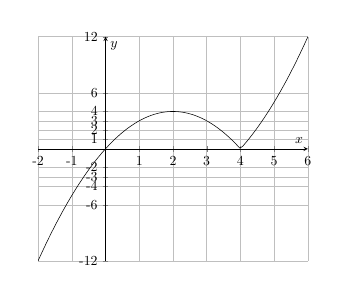
\begin{tikzpicture}[scale=0.5]
\begin{axis}[
    axis lines = middle,
    grid=major,
    legend pos={south west},
    xlabel = {$x$},
    ylabel = {$y$},
    ymin=-12,
    ymax=12,
    xmin=-2,
    xtick={-1,1,3,5,2,-2,4,6},
    xticklabels={-1,1,3,5,2,-2,4,6},
    ytick={ -12,6, 2,-6, -2,1,4,-4,3,-3,12},
    yticklabels={-12, 6, 2,-6, -2,1,4,-4,3,-3,12}           ]
	\addplot[domain=-2:6, samples=100, color=black] {x*abs(4-x)};
%\addplot[domain=-3:5, samples=100, color=black] {-abs(x-1)};
%\addplot[domain=-3.1:2.5, samples=100, color=red] {70*abs(1-2*abs(abs(x)-2))-10*x^2+10*x-70};
	%\addlegendentry{$\text{Рис. 1}$};
\end{axis}
\end{tikzpicture}$$
b) График функции $y=ax-2$ всегда проходит через точку $(0;-2).$ Одну точку пересечения с исходной функцией он имеет только если проходит через точку $(4;0),$ значит  $4a-2=0,\ a=\cfrac{1}{2}.$\\
